\begin{frame}
  \frametitle{Installing Charm}
  \begin{itemize}
    \item Downloading Charm
    \begin{itemize}
      \item \texttt{git clone git://charm.cs.illinois.edu/charm.git}
    \end{itemize}
    \item Building Charm
    \begin{itemize}
      \item \texttt{./build <TARGET> <TARGET ARCHITECTURE> [OPTIONS]}
      \item Net with 64 bit Linux 
      \begin{itemize}
        \item \texttt{./build charm++ net-linux-x86\_64}
      \end{itemize}
      \item Net with 64 bit Linux shared memory (SMP)
      \begin{itemize}
        \item \texttt{./build charm++ net-linux-x86\_64 smp}
      \end{itemize}
      \item Optimized build
      \begin{itemize}
        \item \texttt{./build charm++ net-linux-x86\_64 -with-production}
      \end{itemize}
      \item Ibverbs with 64 bit Linux 
      \begin{itemize}
        \item \texttt{./build charm++ net-linux-x86\_64 ibverbs}
      \end{itemize}
      \item MPI with 64 bit Linux
      \begin{itemize}
        \item \texttt{./build charm++ mpi-linux-x86\_64}
      \end{itemize}
    \end{itemize}
  \end{itemize}
\end{frame}

\begin{frame}
  \frametitle{Compiling a Charm++ Program}
  \begin{center}
    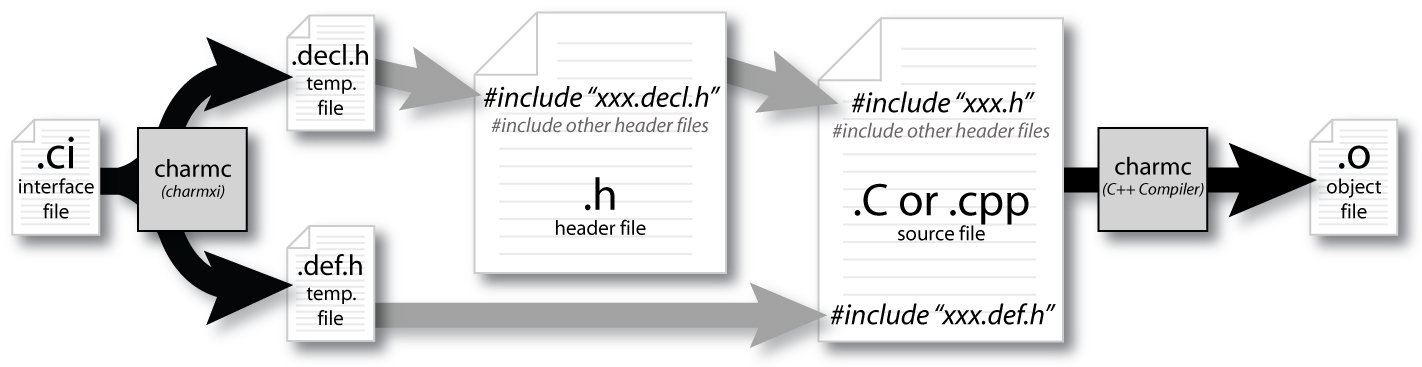
\includegraphics[width=0.9\textwidth]{figures/charmCompile.jpg}
  \end{center}
  \begin{itemize}
    \item Compiling Hello World Example
    \begin{itemize}
      \item \texttt{charmc hello.ci}
      \item \texttt{charmc -c hello.cpp}
      \item \texttt{charmc -o hello hello.o}
    \end{itemize}
  \end{itemize}
\end{frame}

\begin{frame}
  \frametitle{Running a Charm++ Program}
  \begin{itemize}
    \item Run commands
    \begin{itemize}
      \item \texttt{./charmrun +p7 ./pgm}
      \item The \texttt{+p7} tells the system to use seven cores
    \end{itemize}
    \item In debug mode
    \begin{itemize}
      \item Compile with \texttt{-g} option
      \item \texttt{./charmrun +p7 ./pgm ++debug}
      \item Runs each node under gdb in an xterm window
    \end{itemize}
    \item In SMP mode
    \begin{itemize}
      \item \texttt{./charmrun +p14 ./pgm +ppn 7 +pemap 1-7 +commap 0}
      \item \texttt{+ppn} tells the number of pes per node
      \item \texttt{+pemap} binds execution threads to sequence of cores
      \item \texttt{+commap} binds communication threads to the listed cores
    \end{itemize}
  \end{itemize}
\end{frame}


\begin{frame}
  \frametitle{Running ChaNGa}
  \begin{itemize}
    \item Compile
    \begin{itemize}
      \item \texttt{git clone git://charm.cs.illinois.edu/cosmo/changa.git}
      \item \texttt{git clone git://charm.cs.illinois.edu/cosmo/utility.git}
      \item \texttt{cd changa}
      \item \texttt{./configure CHARM\_DIR=<path\_to\_charm>}
      \item \texttt{make -j4}
    \end{itemize}
    \item Run
    \begin{itemize}
      \item \texttt{Download the dataset}
      \item \texttt{./charmrun +p1024 ./ChaNGa -D 1 -ppc 125 -p 52000 -killat 2 ./dwf1.2048.param
      +balancer Orb3dLB\_notopo +LBPeriod 0.1 +LBCommOff +noAnytimeMigration}
    \end{itemize}
  \end{itemize}
\end{frame}

